\subsection{Path Planning}
The path planning consist of two actions, finding a path with A\text{*} and then calculating coordinate targets in the map. 
A\text{*} uses a know map, an initial position, the goal and a cost map to plan out the path to the goal. 
The internal functionality of the A\text{*} function generates a heuristic map based on the goal and the know map. The implementation of A\text{*} is based upon the implementation from the Artificial Intelligence in Robotics Udacity course\citep{AIROK}.\\
The output of the A\text{*} is a path and a policy vector. The policy vector is used to calculate some coordinate targets which are used as targets when the robot moves towards the goal. An example of a plan can be seen in figure \ref{fig:exastar} where start is [ 1 1 ] and the goal is [ 6 5 ]. For a real world example see the results section.
\begin{figure}[H]
\centering
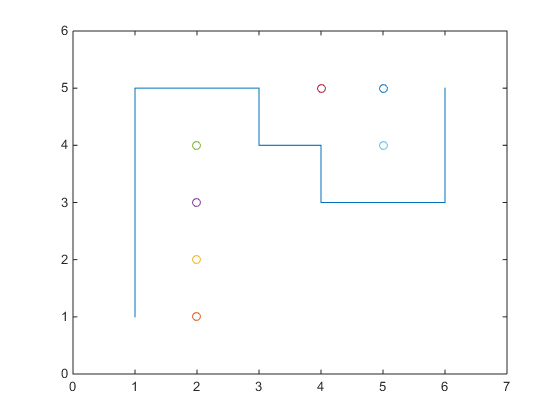
\includegraphics[width=0.5\textwidth]{billeder/exampleastar}
\caption{Example of A star plan}
\label{fig:exastar}
\end{figure}